\documentclass[12pt,a4paper]{article}
\usepackage{graphics}
\usepackage{amssymb}
\usepackage{ragged2e}
\justifying
\usepackage[utf8]{inputenc}
\usepackage[russian]{babel}
\usepackage[width=17cm,top=1cm,height=27cm]{geometry}
\usepackage{graphicx}
\title{Численные методы(Мусаева)}

\date{November 2019}

\begin{document}
\begin{titlepage}
\begin{center}
2019 год
\vspace {8cm}

{ \LARGEПрактикум по численным методам:\\ аппроксимация функций }\\
\vspace {8cm}
\bigskip Мусаева Аида, группа 301
\end{center}
\vfill
\vfill
\end{titlepage}

\section{Метод наименьших квадратов}
\text{Пусть на отрезке $[a,b]$ задана функция $f = (x+3)cos(x)$, причём её значения $\left\{y_i = f(x_i)\right\}$ в узлах сетки $\left\{x_0, x_1, \ldots, x_n\right\}$ известны с погрешностями $\left\{\epsilon_i\right\}$, то есть вместо набора значений
$\left\{y_i\right\}$ имеем $\left\{\widetilde{y} = y_i + \epsilon_i\right\}$. Пусть, кроме того, на $[a,b]$ определены функции $\phi_j, j = \overline{0,m}$
Введём в рассмотрение обобщённый полином:
$P_m(x) = \sum\limits_{j=0}^m{a_j\phi_j}$
Пусть $a$– вектор коэффициентов полинома $P_m$, $y$ – вектор значений функции $f$ и $\phi$ – вектор-функция, составленная из значений $\left\{\phi_j(x)\right\}$:\\\\
$a = (a_0, \ldots , a_m)^T$\\
$y = (y_0,\ldots, y_n)^T$\\
$\phi(x) = (\phi_0(x), \ldots, \phi_m(x))^T$
}
\begin{displaymath}
\mathbf{Q} =
\left( \begin{array}{cccc}
\phi_0(x_0) & \phi_1(x_0) & . . . & \phi_m(x_0) \\
\phi_0(x_1) & \phi_1(x_1) & . . . & \phi_m(x_1) \\
. . . & . . . & . . . & . . . \\
\phi_0(x_n) & \phi_1(x_n) & . . . & \phi_m(x_n)
\end{array} \right)
\end{displaymath}

Для определения параметров искомого полинома нужно решить систему уравнений $Ha=b$, где $H=Q^TQ$, $b=Q^Ty$.

\section{Построение алгебраического полинома наилучшего приближения }
Для выбранной системы ортогональных многочленов $ \left\{ Q_0(x),Q_1(x), ... Q_n(x) \right\} $ многочлен наилучшего приближения $\overline{Q_n}(x)$ запишется в виде:\\

$\overline{Q_n}(x)=c_0Q_0(x)+c_1Q_1(x) + ... + c_nQ_n(x)$,
причём коэффициенты $\left\{c_i\right\}$ вычисляются по формулам: \\
$c_k= \frac{\int_a^b p(x)f(x)Q_k(x)dx}{\int_a^b p(x)Q_k^2(x)dx}$.\\
Частным случаем ортогональных полиномов являются многочлены Лежандра:
$p(x)=1 x\in[-1,1]$, $L_n(x)=\frac{1}{n!2^n}\frac{d^n}{dx^n}[(1-x^2)^n]$.
\section{Код программы}
\begin{verbatim}
import numpy as np
import matplotlib.pyplot as plt
from sympy import *
import sympy
import math


x = Symbol('x')

def f(x):
    return (x + 3) * np.cos(x)

def leastSquares(func):
    x = Symbol('x')
    def Gauss(A, b):
        n = A.shape[0]
        for i in range(n):
            b[i] /= A[i][i]
            A[i] /= A[i][i]
            for j in range(i + 1, n):
                b[j] -= A[j][i] * b[i]
                A[j] -= A[j][i] * A[i]

        for i in range(n - 1, -1, -1):
            for j in range(i - 1, -1, -1):
                b[j] -= b[i] * A[j][i]
        return b

    def phi(dot):
        return Array([1, x, x ** 2, x ** 3]).subs(x, dot)

    X = np.linspace(-1, 1, 5)
    Q = np.array([[(phi(i))] for i in X]).reshape(5, 4)
    a = Gauss(Q.transpose().dot(Q), Q.transpose().dot(func(X)))
    return a.dot(phi(x))


def approxLegendre(func):
    Q = Array([1, x, (3 * x ** 2 - 1) / 2, (5 * x ** 3 - 3 * x) / 2])
    I1 = Array([integrate(func * Q[i]) for i in range(4)])
    I1 = I1.subs(x, 1) - I1.subs(x, -1)
    I1 = np.array([I1[i].evalf() for i in range(4)])
    I2 = Array([[integrate(Q[i] ** 2, x)] for i in range(4)])
    I2 = np.array(I2.subs(x, 1) - I2.subs(x, -1))
    C = np.array([I1[i] / I2[i] for i in range(4)])
    return C.dot(Q.reshape(4, 1))


def plotCompare(func, leastSq, pLegendre):
    xnew = np.arange(-1, 1.01, 0.01)
    fig1, ax = plt.subplots()
    line1, = ax.plot(xnew, func(xnew),
                     label=func.__name__+ "(x)")

    line2, = ax.plot(xnew, [leastSq.subs(x, xnew[i]) 
        for i in range(np.prod(xnew.shape))],
                     label='lSq Polynomial (x)')
    line3 = ax.plot(xnew, [pLegendre.subs(x, xnew[i]) 
        for i in range(np.prod(xnew.shape))],
                    label='approx by pLegendre (x)')

    ax.legend(loc='upper left')
    plt.show()


lSq = leastSquares(f)
print(lSq)
func = (x + 3) * sympy.cos(x)
pLeg = approxLegendre(func)
print(pLeg)
plotCompare(f, lSq, pLeg)
\end{verbatim}
\section{Результат работы программы}
\begin{verbatim}
P(x) = -0.449707008029646*x**3 - 1.36624791454987*x**2 + 0.990009313897785*x
+ 2.98458579858515
P_L(x) = -0.455152732001166*x**3 - 1.39578867025591*x**2 + 0.990492519985849*x
+ 2.98967584450899
\end{verbatim}
\begin{figure}[h]
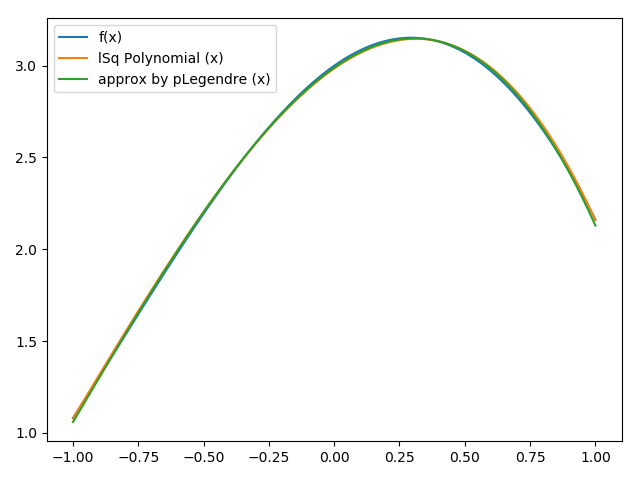
\includegraphics[width=\linewidth]{1.png}
\caption{}
\label{fig:}
\end{figure}\\
\end{document}

\end{document}
